% !TeX root = main.tex


\begin{savequote}[70mm]
,,Z maszyną nie ma dyskusji. Jeśli chce się z~niej korzystać, musi się jej słuchać.''
\qauthor{Antoni Kępiński -- Rytm życia}
\end{savequote}


\chapter{Baza sprzętowa}
\label{chap:sprzet}

%%%%%%%%%%%%%%%%%%%%%%%%%%%%%%%%%%%%%%%%%%%%%%%%%%%%%%%%%%%%%%%%%%%%%%%%%%%%%%%%
%%%%%%%%%%%%%%%%%%%%%%%%%%%%%%%%%%%%%%%%%%%%%%%%%%%%%%%%%%%%%%%%%%%%%%%%%%%%%%%%

\section{Robot mobilny Elektron}

Robot mobilny Elektron powstał w~roku 2007 jako efekt współpracy Instytutu Automatyki
i~Robotyki oraz Instytutu Automatyki i~Informatyki Stosowanej Politechniki Warszawskiej
\cite{SzynkiewiczEtal06}. Został zaprojektowany jako platforma laboratoryjna,
przeznaczona do badań nad systemami sterowania i~nawigacji robotów mobilnych,
czemu sprzyjać miała modułowa konstrukcja zarówno części mechanicznej, jak i~systemu
sterowania. Od momentu powstania robot poddawany był kolejnym modernizacjom,
mającym na celu zarówno dołączenie nowych zestawów czujników, jak i~umożliwienie
sterowania robota przy wykorzystaniu nowych struktur programowych. Pierwotnie Elektron
sterowany był przy wykorzystaniu środowiska Player/Stage, w~ramach niniejszej pracy
robot został uruchomiony wykorzystując system ROS (więcej na ten temat
w~rozdziale~\ref{chap:programowanie}).


\begin{figure}[h!]
\centering
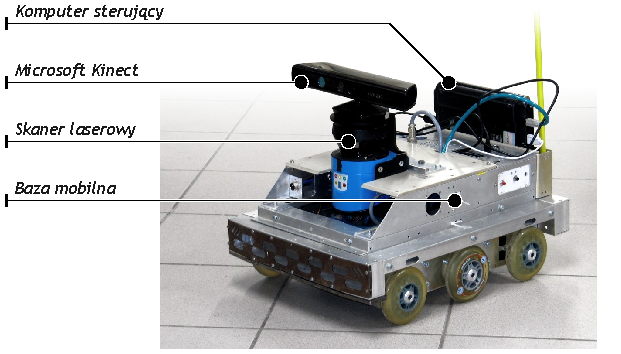
\includegraphics{../../Common/img/elektron/elektron_desc}
\caption[Robot mobilny Elektron]{Robot mobilny Elektron ze wstępnie zamocowanym
sensorem Kinect.}
\label{fig:elektron}
\end{figure}

%-------------------------------------------------------------------------------
\subsection{Konstrukcja mechaniczna}
%-------------------------------------------------------------------------------

Baza jezdna robota jest sześciokołową platformą o~napędzie różnicowym na wszystkie
koła. Robot ma budowę modułową i~w jej skład wchodzą moduły: napędowy (monolityczny
blok zawierający silnik, przekładnię, trzy połączone koła oraz enkoder mierzący
ich położenie), rama centralna umożliwiająca szybki montaż dodatkowych modułów oraz
dwa niezbędne moduły elektroniczne - sekcja zasilania oraz sterowania. Bazowe podwozie
wykonane jest w~całości z~profili aluminiowych, ma wymiary 500x380x220mm i~całkowicie
osłania wszystkie wewnętrzne systemy robota.

\begin{table}[h!]
\caption{Parametry robota Elektron}
\centering
\small
\begin{tabular*}{0.6\textwidth}{@{\extracolsep{\fill}} lr}
\toprule
\textbf{Właściwości kinematyczne}\\
\midrule
Maksymalna prędkość liniowa & 0.25m/s \\
Maksymalna prędkość kątowa & 85\textdegree/s\\
\midrule
\textbf{Zasilanie} \\
\midrule
Pojemność akumulatorów & 2x7200mAh \\
Napięcie akumulatorów & 2x12V \\
Dostępne napięcia & 5V, 12V, 24V \\
Dodatkowe & zintegrowana ładowarka \\
\bottomrule
\end{tabular*}
\label{tab:robot_params}
\end{table}

Pierwotnie komputer sterujący robotem był umieszczony wewnątrz ramy (był to komputer
przemysłowy z~procesorem klasy Pentium III), obecnie do sterowania wykorzystywany
jest netbook EeePC mocowany z~tyłu robota.

%-------------------------------------------------------------------------------
\subsection{Moduły sensoryczne}
%-------------------------------------------------------------------------------

Robot Elektron wyposażony jest w~kilka niezależnych zestawów czujników. Przy realizacji
zadania wykorzystane zostały: układ pomiaru odometrycznego, układ zawierający żyroskop,
układ kamery trójwymiarowej w~postaci urządzenia Microsoft Kienct oraz skaner laserowy
Sick LMS100. Układ pomiaru odometrycznego składa się z~dwóch enkoderów optycznych
umieszczonych w~module napędowym. Każdy z~nich jest w~stanie zmierzyć kąt obrotu kół
napędowych z~rozdzielczością 4000 impulsów na obrót. W~projekcie zrezygnowano z~montowania
dodatkowych czujników na wałach silników.

Drugi z~wymienionych układów służy do pomiaru prędkości kątowej w~celu wspomagania
obliczeń położenia i~orientacji robota. Zawiera żyroskop Analog Devices ADXRS401,
połączony z~mikrokomputerem jednoukładowym PIC16F688, przy pomocy którego pomiary
przekazywane są do komputera sterującego za pomocą interfejsu USB.

% TODO: Sprawdzić model mikrokontrolera na płytce z~żyroskopem

\begin{table}[h!]
\caption{Parametry żyroskopu ADXRS401}
\centering
\small
\begin{tabular*}{0.6\textwidth}{@{\extracolsep{\fill}} lr}
\toprule
\textbf{Czułość}\\
\midrule
Zakres pracy & \textpm 75\textdegree/s \\
Współczynnik skali & 12.75 - 17.25 mV/\textdegree/s \\
\midrule
\textbf{Temperatura pracy} \\
\midrule
Zakres temperatur & -40 - +85\textdegree C \\
Współczynnik temperaturowy & 8.5mV/K \\
\bottomrule
\end{tabular*}
\label{tab:gyro_params}
\end{table}


%%%%%%%%%%%%%%%%%%%%%%%%%%%%%%%%%%%%%%%%%%%%%%%%%%%%%%%%%%%%%%%%%%%%%%%%%%%%%%%%
%%%%%%%%%%%%%%%%%%%%%%%%%%%%%%%%%%%%%%%%%%%%%%%%%%%%%%%%%%%%%%%%%%%%%%%%%%%%%%%%

\section{Microsoft Kinect}

Jest to kontroler do gier dla konsoli Xbox wykorzystujący analizę światła
strukturalnego. Pomimo jego pierwotnego przeznaczenia, kilka dni po premierze
został opublikowany nieoficjalny sterownik umożliwiający wykorzystanie
informacji z~jego czujników na komputerze PC~\cite{Giles201022}. Jego niska cena
(500PLN), dostępność wielu algorytmów ułatwiających wykorzystanie dostarczanych
przez niego informacji oraz szybkość i~dokładność działania sprawiły, że został
on wybrany jako główne źródło informacji o~scenie do wykorzystania w~projekcie.

\begin{figure}[h!]
\centering
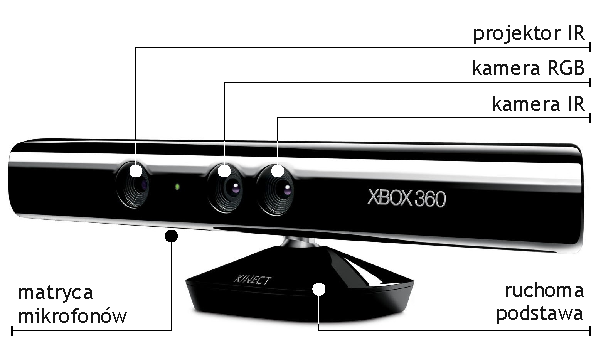
\includegraphics{../img/kinect_hardware}
\caption[Sensor Kinect firmy Microsoft]{Sensor Kinect firmy Microsoft z~zaznaczonymi
kluczowymi elementami.}
\label{fig:kinect_hardware}
\end{figure}

%-------------------------------------------------------------------------------
\subsection{Budowa}
%-------------------------------------------------------------------------------

Kluczowe elementy sensora Kinect zaznaczone są na rysunku~\ref{fig:kinect_hardware}.
Pomiar głębi realizowany jest przy użyciu pary złożonej z~projektora podczerwieni
oraz kamery rejestrującej obraz w~tym paśmie. Kamera RGB umieszczona pomiędzy nimi
służy do rejestracji widocznej sceny, a~dzięki jej kalibracji z~pomiarem głębi
możliwe jest tworzenie trójwymiarowych map otoczenia z~nałożoną teksturą (dane
kalibracyjne dostarczone przez producenta są zapisane bezpośrednio w~urządzeniu).

\begin{figure}[h!]
\centering
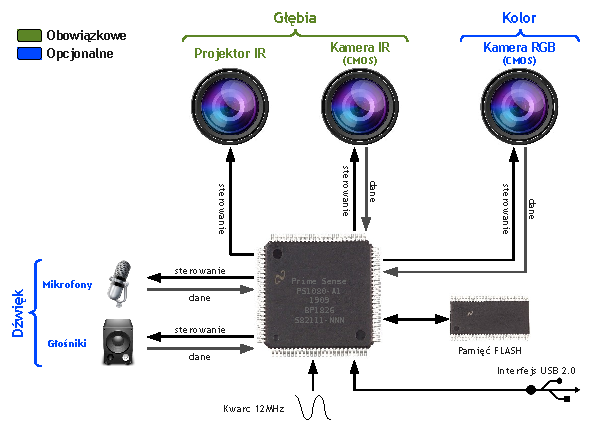
\includegraphics{../../Common/img/primesense}
\caption{Schemat blokowy sensora Kinect}
\label{fig:kinect_block}
\end{figure}

Dodatkowo Kinect wyposażony jest w~matrycę czterech mikrofonów, które mogą być
wykorzystane do lokalizacji źródeł dźwięku w~przestrzeni, a~także podstawę umożliwiającą
pochylanie sensora w~zakresie~27\textdegree~w~górę i~w~dół.

Istotne parametry techniczne zebrane są w~tabeli~\ref{tab:kinect_params}.

\begin{table}[h!]
\caption{Kinect -- parametry techniczne}
\centering
\small
\begin{tabular*}{0.6\textwidth}{@{\extracolsep{\fill}} lr}
\toprule
\textbf{Pole widzenia}\\
\midrule
Poziome & 57\textdegree \\
Pionowe & 43\textdegree \\
Zakres ruchu góra/dół & $\pm$27\textdegree \\
Efektywny pomiar odległości & 1.2m - 3.5m \\
\midrule
\textbf{Kamera RGB} \\
\midrule
Rozdzielczość & 640x480px \\
Głębia & 8 bitów \\
Częstotliwość akwizycji & 30kl/s \\
\midrule
\textbf{Mapa głębi} \\
\midrule
Rozdzielczość & 320x240px \\
Głębia & 16 bitów \\
Częstotliwość akwizycji & 30kl/s \\
\bottomrule
\end{tabular*}
\label{tab:kinect_params}
\end{table}

%-------------------------------------------------------------------------------
\subsection{Działanie}
%-------------------------------------------------------------------------------

Sercem urządzenia jest dedykowany układ tworzący mapę głębi na podstawie analizy
obrazu z~kamery IR. W~pierwszym kroku na scenę rzutowany jest specjalny wzór
(przedstawiony na rysunku~\ref{fig:kinect_pattern}), a~uzyskany obraz jest
rejestrowany przez kamerę działającą w~paśmie bliskiej podczerwieni.

\begin{figure}[h!]
\centering
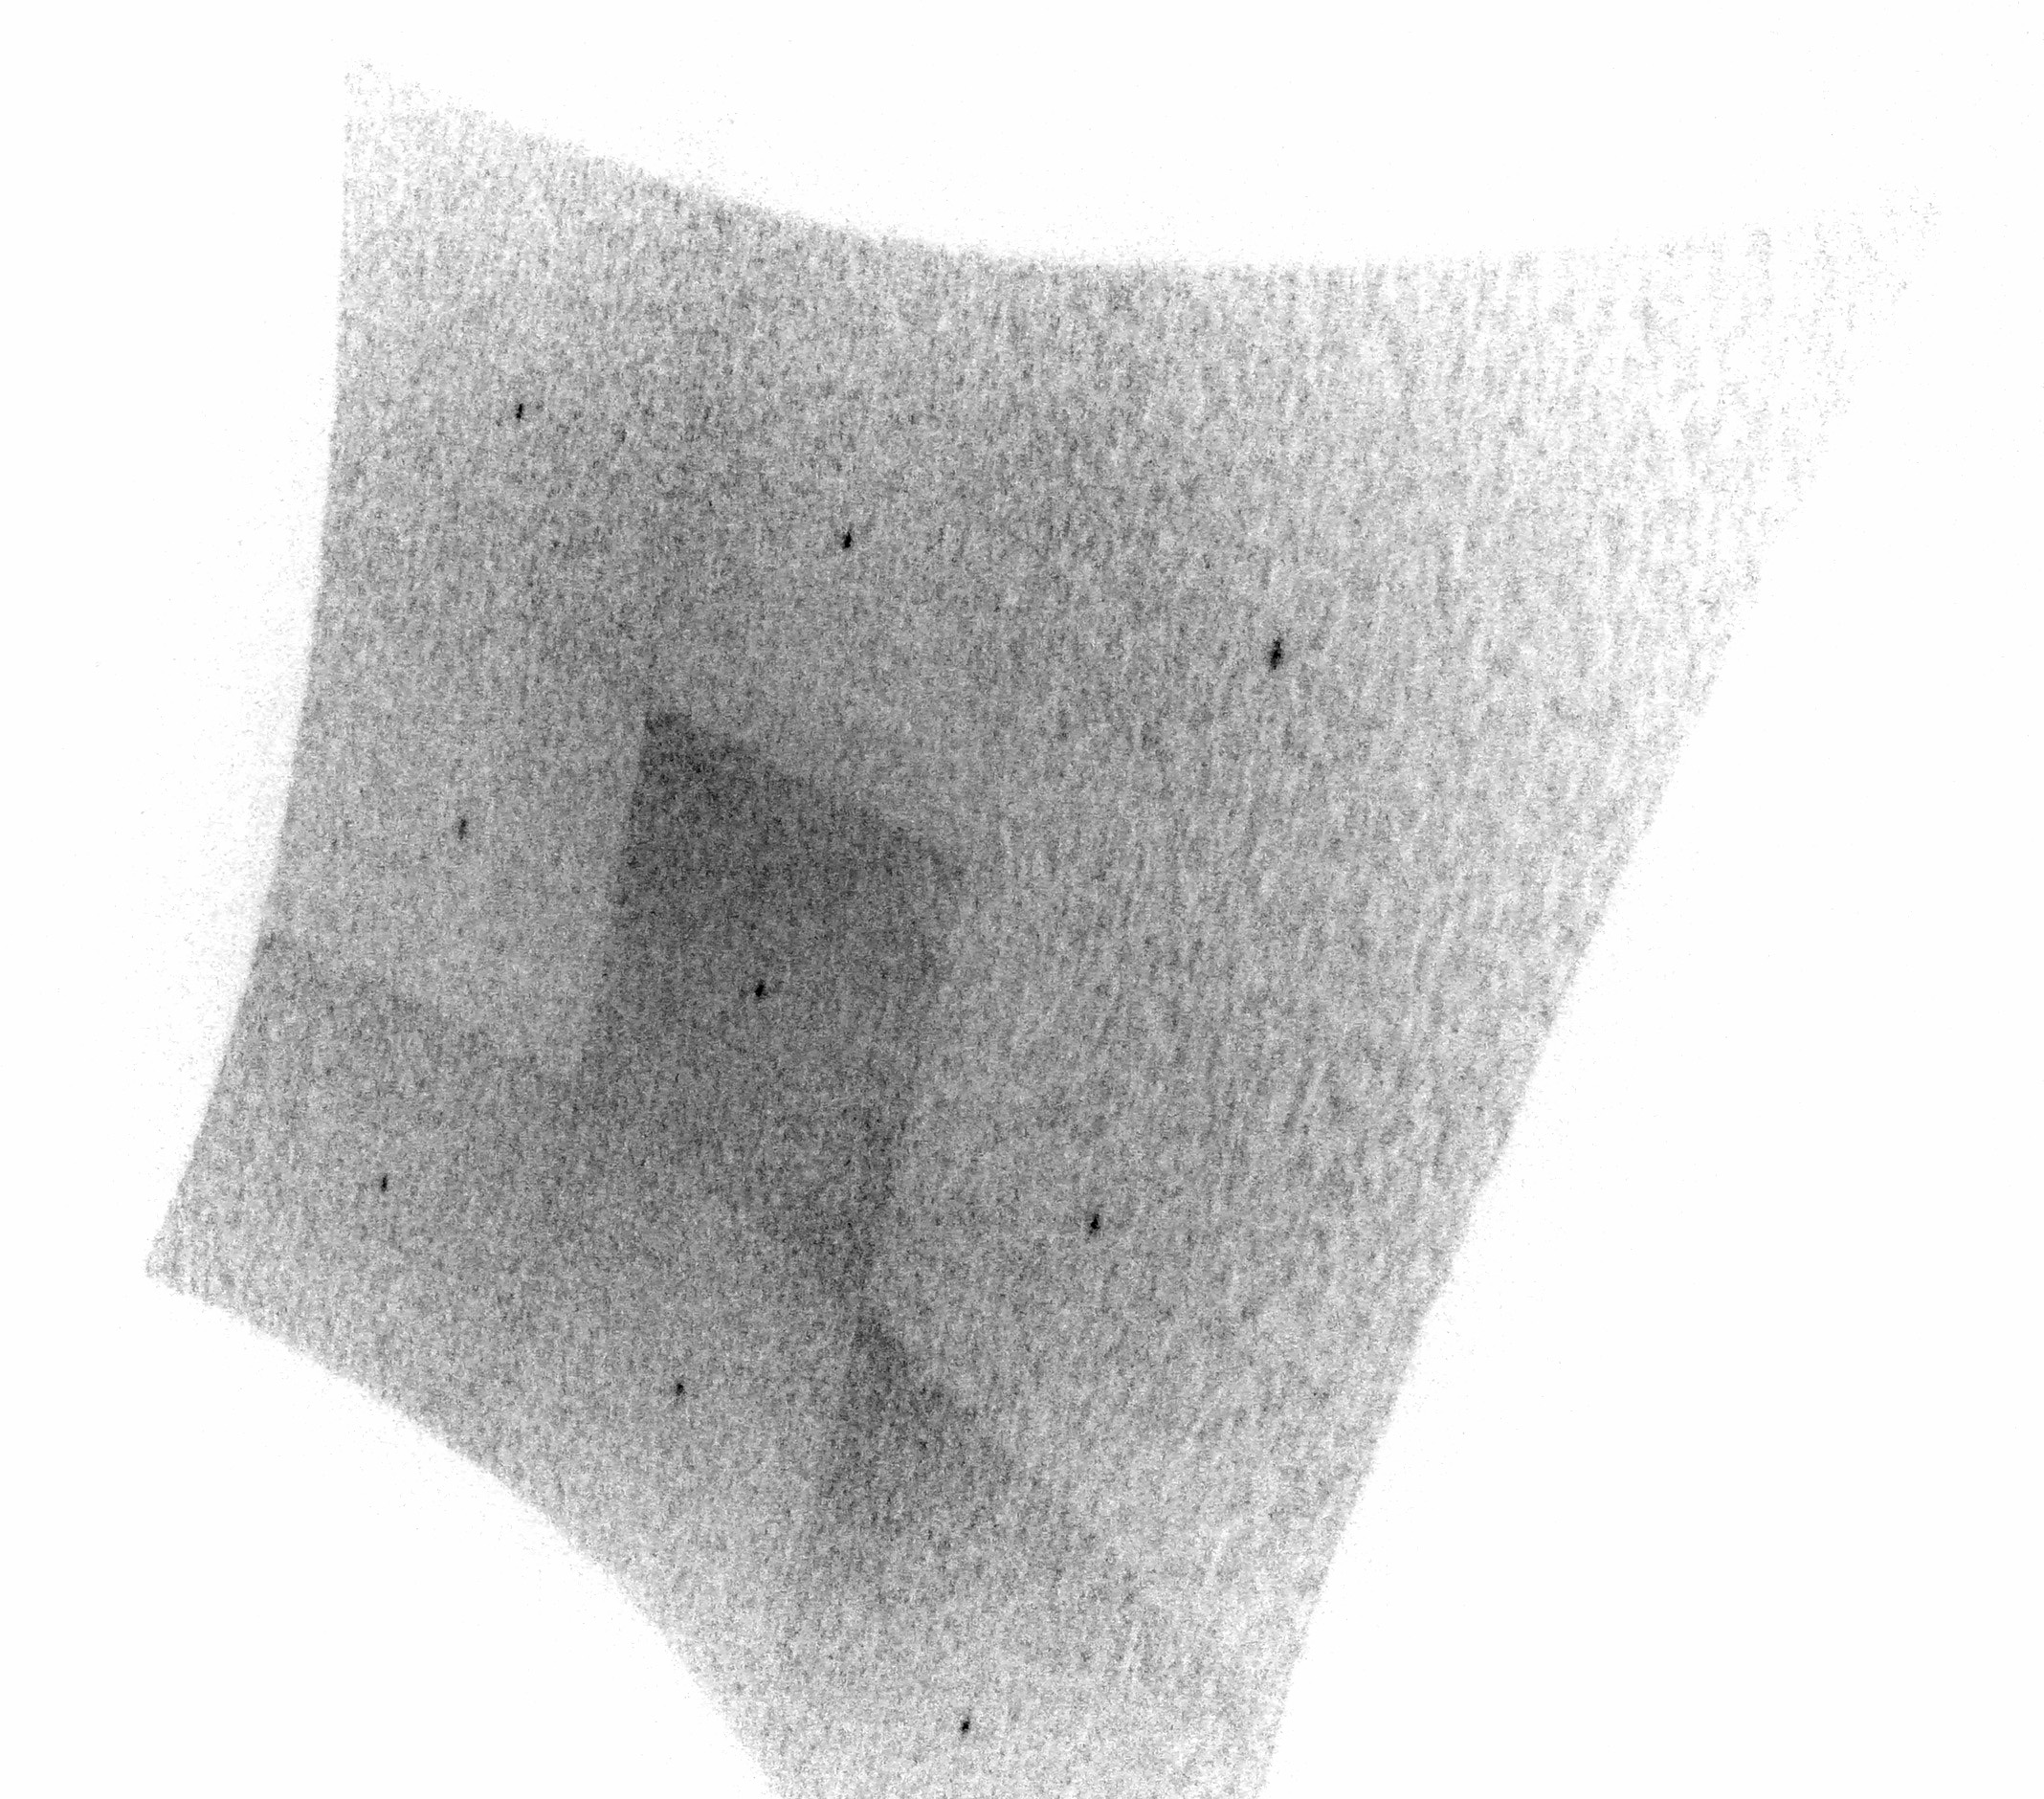
\includegraphics[width=8cm]{../img/kinect_pattern}
\caption[Wzór rzucany przez Kinect]{Wzór rzucany przez Kinect (kolory odwrócone,
ciemne punkty oznaczają miejsca oświetlane przez rzutnik podczerwieni). Źródło:
http://goo.gl/L7sJm}
\label{fig:kinect_pattern}
\end{figure}

Wzór ma specjalną strukturę, umożliwiającą poprawne zlokalizowanie analizowanych
pikseli w~obrazie wzorcowym bez konieczności wielokrotnego rzutowania różnych
tekstur (tak jak przy metodzie wykorzystującej kod Graya i~coraz węższe paski).
Zaczynając od największych bloków wyróżnić w~nim można szachownicę 3x3 pola,
a~na środku każdego z~nich jaśniejszy punkt służący do lokalizacji centrum danego
segmentu. Każde z~pól pokryte jest siatką punktów ułożonych w~taki sposób, aby
ich bloki powtarzały się bardzo rzadko lub wcale w~obrębie danego pola
szachownicy (w ten sposób wyeliminowany został problem fałszywych dopasowań
podczas porównywania z~obrazem referencyjnym). Po zlokalizowaniu pozycji
pikseli w~mapie wzorcowej z~triangulacji wyliczane jest ich względne
przesunięcie, a~z niego ostateczna mapa głębi.

%-------------------------------------------------------------------------------
\subsection{Mocowanie na robocie}
%-------------------------------------------------------------------------------

Mocując sensor na robocie należało uwzględnić ograniczoną minimalną odległość,
z~jakiej Kinect wykrywa obiekty. Początkowo urządzenie zostało zamocowane na
dole robota, przed skanerem laserowym. Rozwiązanie to miało jednak dwie wady --
po pierwsze obiekty znajdujące się bliżej niż 60cm od robota nie były
wykrywane, po drugie oś optyczna sensora była pod tak ostrym kątem do podłogi,
że nie była ona praktycznie wykrywana. Na rysunku~\ref{fig:elektron} pokazana
jest druga próba mocowania, na głowicy lasera, ale okazało się, że i~taka
wysokość nie jest wystarczająca, aby w~pełni wykrywać obiekty przed robotem.
Ostatecznie sensor zamocowany jest bliżej tylnej części robota, kilka
centymetrów powyżej skanera Sick, i~jest pochylony o~20\textdegree w~dół. Taka
konfiguracja umożliwia wykrywanie przeszkód w~całym pasie przed robotem,
znajdujących się nie bliżej niż 10cm od jego przedniej krawędzi.
Rysunek~\ref{fig:range} przedstawia ostateczne umiejscowienie czujników
na robocie, wraz z~zaznaczonymi polami widzenia Kinecta i~skanera laserowego.

% TODO: Stworzyć schemat elektrona z~zamocowanym kinectem i~pokazanym polem
% widzenia kinecta i~sicka


\begin{figure}[htb!]
\centering
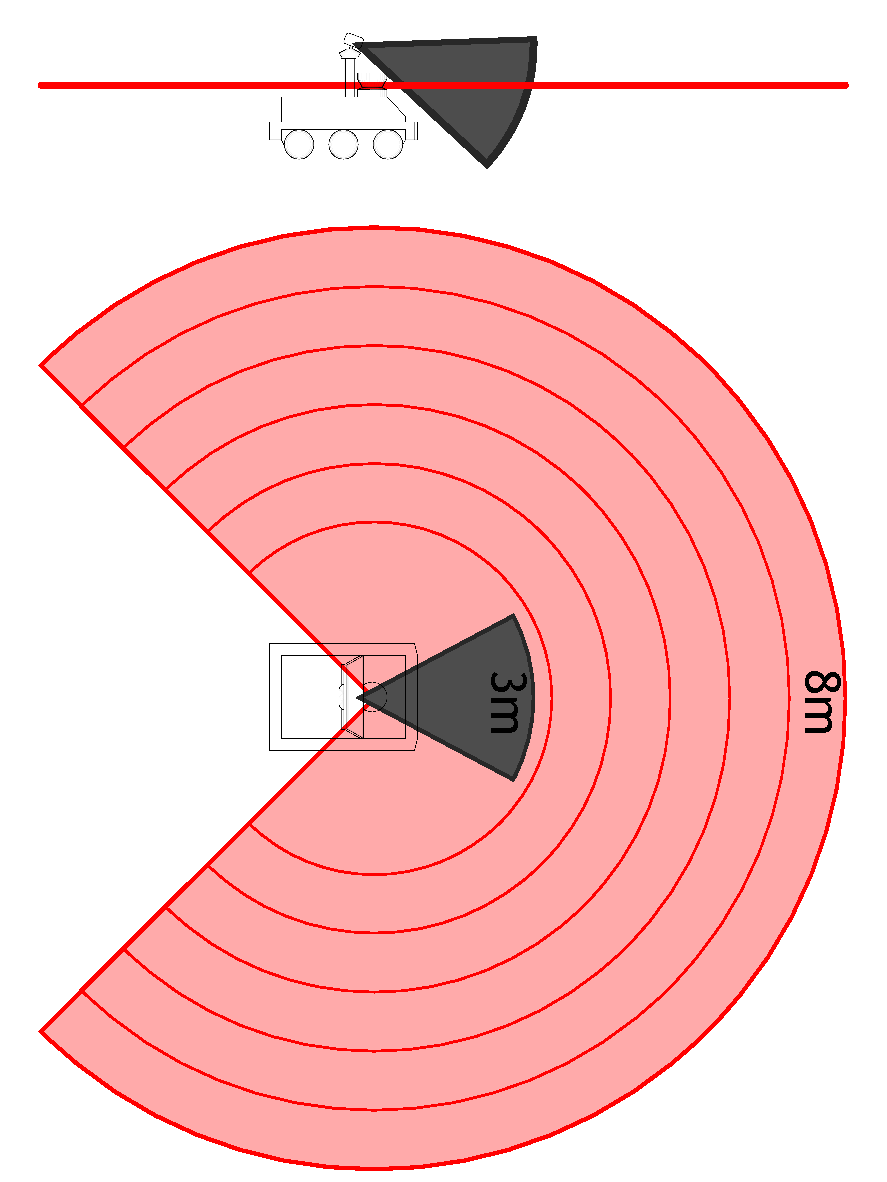
\includegraphics[width=8cm]{../../Common/img/elektron/range}
\caption[Przybliżone zasięgi działania czujników umieszczonych na robocie
Elektron]{Przybliżone zasięgi działania czujników umieszczonych na robocie
Elektron. Odcieniem jaśniejszym oznaczono efektywne pole działania skanera Sick,
ciemniejszym zasięg sensora Kinect. Dla czytelności rysunek samego robota
jest w~skali większej niż pokazane zasięgi.}
\label{fig:range}
\end{figure}


%%%%%%%%%%%%%%%%%%%%%%%%%%%%%%%%%%%%%%%%%%%%%%%%%%%%%%%%%%%%%%%%%%%%%%%%%%%%%%%%
%%%%%%%%%%%%%%%%%%%%%%%%%%%%%%%%%%%%%%%%%%%%%%%%%%%%%%%%%%%%%%%%%%%%%%%%%%%%%%%%

\section{Skaner laserowy SICK LMS100}

Skaner laserowy firmy Sick, model LMS100 jest urządzeniem zdolnym do mierzenia
odległości do otaczających obiektów w~zakresie 270\textdegree. Pomiar dokonywany
jest przy użyciu promienia lasera, który odbijany jest od obracającego się
lustra. Po odbiciu od przeszkody dokonywany jest pomiar czasu, po jakim wiązka
wróciła do detektora, a~z tego wyliczana jest odległość. W~przypadku modelu
LMS100 dla każdego promienia dokonywane są faktycznie dwa pomiary, dzięki czemu
dużo rzadziej zdarzają się zafałszowane wyniki (spowodowane np. odbiciem
promienia od kropli deszczu), dodatkowo wraz z~odległością każdy pomiar ma
dołączoną intensywność wracającego światła (to z~kolei pozwala np. wykrywać
szyby znajdujące się przed robotem -- powodują one powrót pierwszego impulsu
o~niskim natężeniu).

\begin{figure}[h!]
\centering
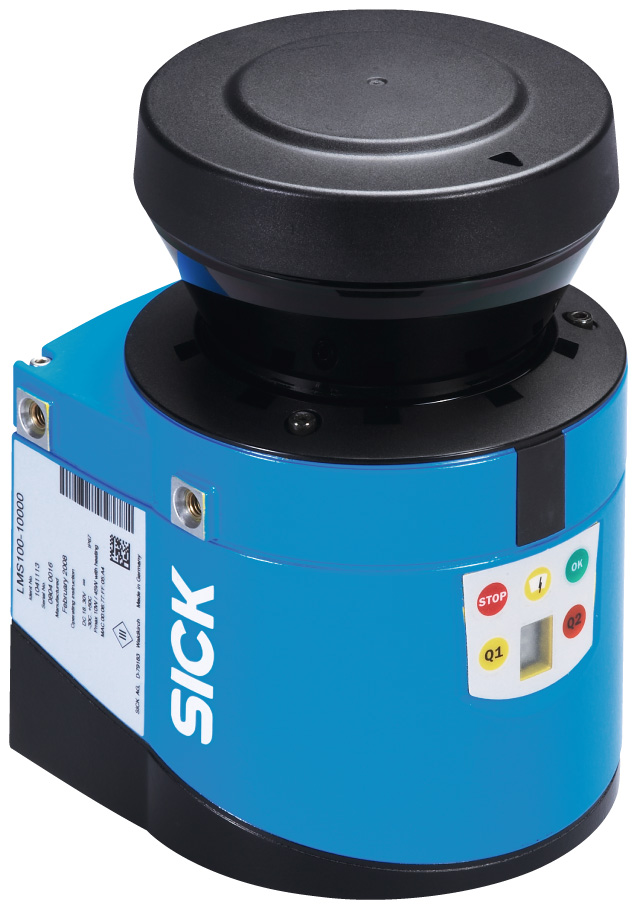
\includegraphics[height=5cm]{../img/LMS100}
\caption{Skaner laserowy SICK LMS100}
\label{fig:sick}
\end{figure}

Początkowo na robocie Elektron zamontowany był skaner laserowy Sick LMS200
(pokazany na rysunku~\ref{fig:sick_obrotnica}), jednak z~powodu jego wielkości
utrudnione było montowanie dodatkowych elementów na korpusie robota. Dlatego też
został on zastąpiony mniejszymi skanerami LMS100, które dodatkowo mają
korzystniejsze parametry techniczne przy wykorzystaniu na robotach mobilnych
operujących w~pomieszczeniach zamkniętych (ich zestawienie zebrane
w~tabeli~\ref{tab:sick_params}).

\begin{table}[h!]
\caption{Parametry skanerów laserowych Sick LMS100 i LMS200}
\centering
\small
\begin{tabular*}{0.8\textwidth}{@{\extracolsep{\fill}} lcc}
\toprule
\textbf{Parametry skanu} & LMS100 & LMS200\\
\midrule
Zasięg & 10m & 20m \\
Rozdzielczość kątowa & 0.25\textdegree / 0.5\textdegree & 0.25\textdegree /
0.5\textdegree / 1\textdegree \\
Kąt skanowania & 270\textdegree / 270\textdegree & 100\textdegree /
180\textdegree / 180\textdegree \\
Częstotliwość skanowania & 25Hz / 50Hz & 18Hz / 37Hz / 75Hz \\
\midrule
\textbf{Inne} \\
\midrule
Interfejs komunikacyjny & ethernet 100Mbps & RS232/422 max. 0.5Mbps \\
Pobór mocy & 12W & 20W\\
Masa & 1.1kg & 4.5kg\\
\bottomrule
\end{tabular*}
\label{tab:sick_params}
\end{table}

\subsection{Mocowanie na robocie}

Skaner zamocowany jest na stałe w~przedniej części robota. Rezygnacja
z~mocowania na obrotowej głowicy umożliwiła jego częściowe wsunięcie do wnętrza,
przez co obniżony został poziom pracy skanera (wykrywane są obiekty na
wysokości zbliżonej do wysokości robota). Sposób zamocowania lasera zobaczyć
można na rysunku~\ref{fig:elektron}.

%%%%%%%%%%%%%%%%%%%%%%%%%%%%%%%%%%%%%%%%%%%%%%%%%%%%%%%%%%%%%%%%%%%%%%%%%%%%%%%%
%%%%%%%%%%%%%%%%%%%%%%%%%%%%%%%%%%%%%%%%%%%%%%%%%%%%%%%%%%%%%%%%%%%%%%%%%%%%%%%%

\section{Komputer sterujący}

Pierwotnie Elektron posiadał zabudowany komputer przemysłowy klasy Pentium III 900MHz.
Był on umieszczony wewnątrz robota, przez co dostęp do niego był lekko utrudniony.
Dodatkową wadą takiego rozwiązania był brak monitora -- podczas pracy w~laboratorium
możliwa była jego obsługa zdalna, jednak wychodząc z~robotem poza laboratorium
konieczne było zabieranie bądź dodatkowego monitora i~klawiatury, bądź laptopa
w~celu jego obsługi. Aby wyeliminować te niedogodności, a~także zwiększyć moc
obliczeniową, komputery przemysłowe zostały zastąpione netbookami Asus Eee PC 901.
Mocowane są one w~tylnej części robota, w~specjalnej kieszeni, przez co jest do
nich łatwy dostęp.

\begin{figure}[h!]
\centering
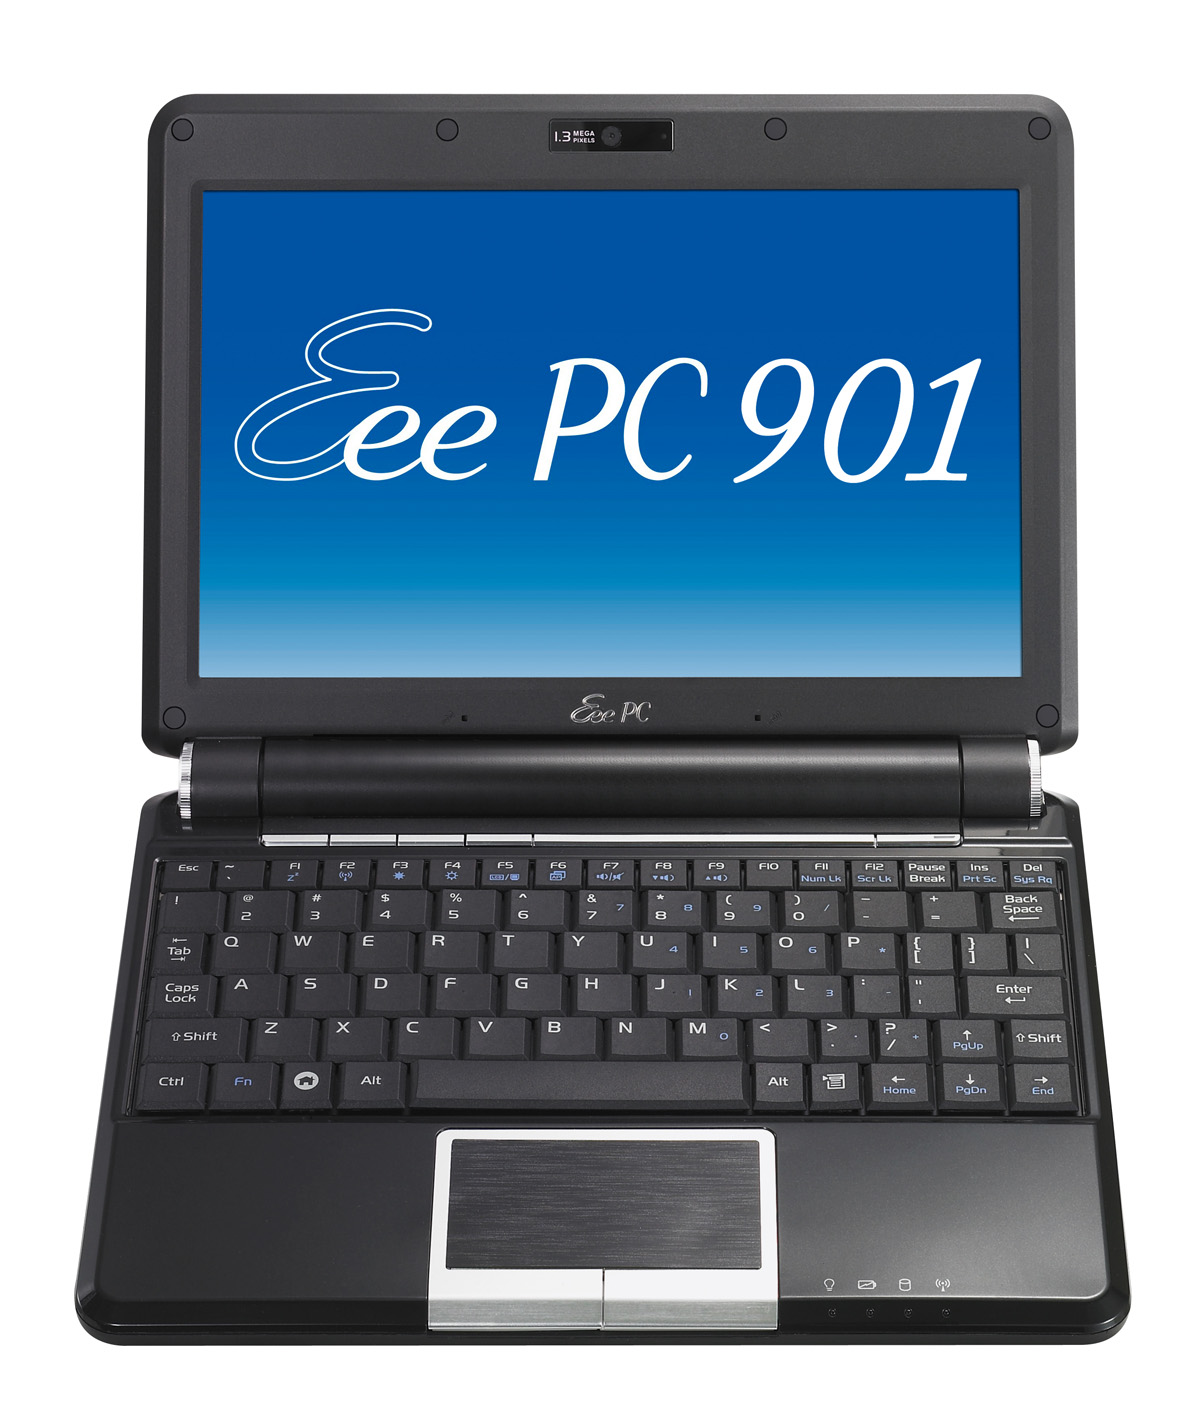
\includegraphics[height=6cm]{../img/eee}
\caption{Netbook Asus Eee PC 901}
\label{fig:eee}
\end{figure}

Konkretny model laptopa wybrany został ze względu na kilka parametrów, z~których
najważniejszymi były wielkość oraz technologia wykonania pamięci masowej. Wybrany
komputer posiada ekran o~przekątnej 8.9", przez co cała konstrukcja jest zwarta
i~niewielka, bez problemów mieszcząc się w~przeznaczonym do tego miejscu (robot
z~zamocowanym komputerem przedstawiony jest na rysunku~\ref{fig:elektron}). W~przypadku
dysku twardego kluczowe było, aby nie posiadał żadnych elementów mechanicznych,
które mogłyby doprowadzić do jego uszkodzenia podczas jazdy robota (nagłe uderzenia
czy nierówności nawierzchni). Pierwszy komputer wyposażony był w~karty pamięci
CompactFlash w~roli dysków twardych, wybrany model laptopa posiada natomiast
dyski twarde wykonane w~technologii SSD. Najważniejsze parametry techniczne
zastosowanych komputerów zebrane są w~tabeli~\ref{tab:eee_params}.
Pomimo, iż moc obliczeniowa nowych komputerów zwiększyła się w~porównaniu
z~rozwiązaniem pierwotnym, to i~tak jest ona niewielka (jak na obecne czasy),
dlatego należy uważnie planować wykorzystywanie czasochłonnych algorytmów
i~w~miarę możliwości wykorzystywać do tego inne maszyny dostępne w~obrębie sieci
WiFi.

\begin{table}[h!]
\caption{Asus Eee PC 901 -- istotne parametry techniczne}
\centering
\small
\begin{tabular*}{0.6\textwidth}{@{\extracolsep{\fill}} lr}
\toprule
\textbf{Procesor}\\
\midrule
Model & Intel Atom N270\\
Taktowanie & 1.6GHz\\
Ilość rdzeni & 1 (2 wątki)\\
Architektura & 32bit \\
\midrule
\textbf{Pamięć RAM} \\
\midrule
Pojemność & 1GB \\
Taktowanie & 667MHz \\
\midrule
\textbf{Pamięć masowa} \\
\midrule
Technologia & SSD \\
Pojemność & 4+8GB \\
\midrule
\textbf{Inne} \\
\midrule
Ciężar & 1.1kg \\
Pojemność akumulatora & 6600mAh \\
\bottomrule
\end{tabular*}
\label{tab:eee_params}
\end{table}


